\chapter{Evaluation}
\label{chap:evaluation}
We implemented the algorithm explained in Chapter \ref{chap:testgeneration} as Eclipse plug--in and successfully tested it for a set of academic problems and performed a case study with a real world model from Airbus. We will point out that the transparent interchangeability of solvers is indeed one of the biggest advantages of the approach presented in this thesis. Also the limitations as well as missing but easily implementable features increasing the usability will be discussed in Section \ref{sec:evaluationLimitations}.\\
\section{Example Models and Case Study}
In order to demonstrate the strength of our approach we built a set of test models. Each test model requires an instance of another mathematical programming problems presented in the \nameref{sec:Maths} to be solved in order to generate test data. For each test model we generated test cases with the depth first search explained in Section \ref{sec:pathsearchDFS} using the early infeasible path eliminiation explained in Section \ref{sec:EarlyInfeasiblePathRecognition}. We explain which problem the mathematical program generated for each test model is an instance of and justify which solvers are suitable to solve it. With each selected solver we generated test cases for the test model using different parameters for the depth first search and early infeasible path recognition. We measured the total runtime of our algororithm and plotted the runtime for differnt parameters graphically.\\
We also build a C-implementation for each academic test model and compiled and ran the generated unit tests against them and manually introduced some errors and checked wheather they are detected by the generated test suite.
\subsection{Runtime Measurement}
The total runtime of our algorith is mainly influenced by two factors: The time necessary to solve one instance of the mathematical problem and the total count of problems to be solved during unit test generation. The total count of problems beeing solved depends on the model and the parameters used for the \nameref{sec:pathsearch}. For an acyclic activity diagram there is a finite number of control flow paths and abstract test cases. Assuming an activity diagram showing a tree like control flow graph of depth 10 and a fanout of two in each node we get a total of $2^{10}$ abstract test cases. With normal breadth first or depth first path seach we will have to solve one mathematical program for each control flow path in order to obtain test data, or find out that it is an infeasible control flow path. In general we can say the number of control flow paths in an activity diagram grows exponentially with the number of decisions in the activity diagram; so does the number of problems beeing solved.\\
For the \nameref{sec:pathsearch} we examine the influence of three parameters on the overall runtime. That is the maximum path length, the maximum number of test cases, and the number of unchecked steps. The maximum path length bounds the path search in depth and ensures the termination of the algorithm. For an activty diagram containing at least two different cycles the number of abstract test cases grows exponentially with the maximum path length. %Assume an activity diagram showing a loop, where in each iteration there is one decision with two possible control flows to take. Not after each node there are multiple outgoing edges, that means not every control flow in the control flow path has been choosen among several options, but the number of coises is linearly related to the maximum path length. Assume for the cyclic activity the cycle with the decision in it has the length of three no matter wich path had been taken inside the loop. 
The total ammount of control flow paths found in a graph with two alternative cycles can be calculated as shown in Equation \ref{eqn:MaxPathLength} where $l_{MAX}$ denotes the maximum path length and $a$ the cycle length
\begin{equation}\sum_{n=1}^{max path length/a}{2^n}\label{eqn:MaxPathLength}\end{equation}
The parameter maximum number of test cases obviously linearly with the number of abstract test cases that need to be checked wheather valid test data can be obtained for them. The count of mathematical problems to be solved is the maximum number of test cases divided by the chance that any abstract test case found is an infeasible path. 
The parameter unchecked steps plays a role, when the early infeasible path recognition is activated. The early infeasible path elimination will cut off a huge amount of abstract test cases when a some sub-path is found to be infeasilbe, but it will also slightly increase the count of problems to be solved in the worst case. We again consider the tree like control flow graph with a fanout of two and a depth of ten. We have to solve one mathematical program for each abstract test case to obtain the test data and during the path search we will solve several a mathematical program for several sub--paths. Assuming all $2^{10}$ abstract test cases are feasible paths the number of problems to be solved is approximately given in Equation (\ref{eqn:infeasiblePathRecognitionWorstCase}). $l_{UNCHCK}$ is the number of unchecked steps.
\begin{equation}
2^{10}+\sum_{n=l_{UNCHCK}+1, \Delta n=l_{UNCHCK}+1}^{10}{2^n}
\label{eqn:infeasiblePathRecognitionWorstCase}
\end{equation}
When we determine already after the third decision one of the $2^3$ control flow sub--paths to be infeasible that will reduce the total number of mathematical programs beeing solved by $\frac{1}{8}$. The less unchecked steps we use the more mathematical problems will be solved in vain if all paths are feasible, but the earlyer we get the chance to eliminate infeasible paths the larger is the fraction of the search space we can directly cut off when an infeasible path is recognized. The optimal value for the unchecked steps parameter is a tradeof between solving unecessarily many mathematical problems and not beeing able to cut of large portions of infeasible abstract test cases early enough.
\\
The runtime of a single solver run for models that require decidable problems with a tractable algorithm to be solved is usually below $0.01$ seconds. Also for problems with intractable algorithms the runtime stays below one second. A slight advantage in terms of solving speed has a large impact on the overall runtime since that is the part that consumes more than 99\% of the overall runtime. For undecidable problems we get the problem, that the heuristig might run forever and we need a good time limit for that. 
We meassured the overall runtime of our algorithm transforming a UML \UMLType{Activity} into a compilable unit test varying the maximum path length, the maximum number of test cases, the number of unchecked steps, the used solver and its options and plottet the graphs for each of the academic example models and the case study.
\subsection{Academic Examples}
\label{sec:evaluationAcademicModels}
We will start with models, which require easy problems to be solved in order to obtain test data. By easy we mean decidable problems with a tractable algorithm. Then we will explain how we generated test data for problems, which require NP-hard problems to be solved. Finally we will also present models, which require an instance of an undecidable problem to be solved in order to obtain test data. That means we can only generate test data for them with heuristic methods.\\
Each solver is suitable for another problem class and for several problem classes there are multiple solvers that could be used. We performed some comparisons of different solvers in terms of runtime and the test data produced. For each presented test model we produced test data for all paths up to some maximum length and examined how much more effort in terms of runtime it is to generate boundary values as test data.\\
Finally we built a C implementation of the function modelled by the input to our algorithm and execute the generated test suite against this implementation. We also manually introduced some errors into the implementation and verified, that the produced test suite contains test cases that fail on those errors and that all test pass when the implementation is correct.
\subsubsection{Triangle Classificator}
\begin{figure}
\includegraphics[width=\textwidth]{./pics/TriangleLIN.pdf}
\caption{Triangle Classificator}
\label{fig:TriangleLin}
\end{figure}
\begin{figure}
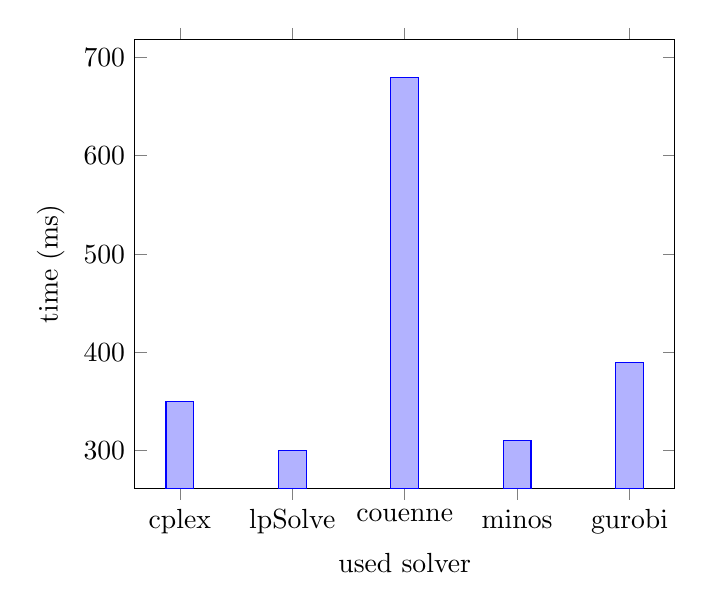
\begin{tikzpicture} 
\begin{axis}[ ybar,
ylabel={time (ms)},
xlabel={used solver},
symbolic x coords={{cplex}, {lpSolve}, {couenne}, {minos}, {gurobi}},
]
\addplot coordinates {(cplex,350) (lpSolve,300) (couenne,680) (minos,310) (gurobi,390)}; 
\end{axis}
\end{tikzpicture}
\caption{Runtime of unit test generation using different solvers}
\label{fig:TriangleLinRuntime}
\end{figure}
We start with a model that contains only linear equalities and inequalities and variables in $\mathbb{R}$. Figure \ref{fig:TriangleLin} shows the activity diagram of a function taking three floating point values as input and returning a floating point value indicating wheather the input variables could possibly be the side lenthes of an equilateral, isoscales, or scalane triangle. The mathematical problem to solve for this model is a linear program and can be solved with the simplex method as implemented in cplex and lp\_solve or an interior point method as implemented by minos and gurobi. And there are many more Solvers available to solve this kind of problem. Generating test data for for every feasible abstract test case takes fore every tested solver less than one second. There are in total 19 possible test cases resulting from this model. Figure \ref{fig:TriangleLinRuntime} shows the average runtime consumed for test generation using different solvers.
\subsubsection{Triangle Classificator with Logical Constraints}
\begin{figure}
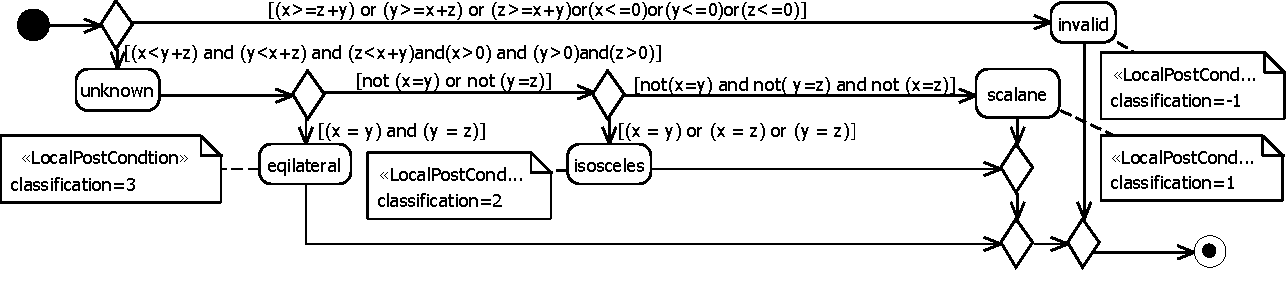
\includegraphics[width=\textwidth]{./pics/TriangleSMT.pdf}
\caption{Activity diagram of a triangle classificator using logical operations}
\label{fig:TriangleSMT}
\end{figure}
Since the formulation of the constraints by means of non-strict inequalities only is not very efficient we reformulated the model and used logical operations as well as strict inequalities in the guards and local post--conditions and yield the model depicted in Figure \ref{fig:TriangleSMT}. The variables are now all in the domain of integers. This model will be transformed into an instance of an satisfiable modulo theories problem. Suitable solvers to solve instances of SMT are geode, ilogcp and jacop. In total there are 4 possible test cases to be found and any of the solver needs less than a second to generate test data for all of them.
\subsubsection{Binary Counter}
\begin{figure}
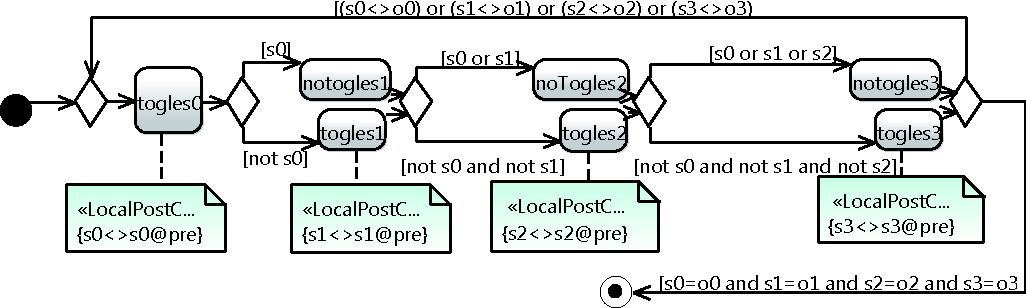
\includegraphics[width=\textwidth]{./pics/BinaryCounter.pdf}
\caption{Activity diagram of a binary counter incrementing a 4 bit register}
\label{fig:BinaryCounter}
\end{figure}
In Figure \ref{fig:BinaryCounter} we depict the activity diagram of a binary counter. The variables $s0$ to $s3$ hold the current state of the counter. The activity models a function with four input arguments $o0$ to $o3$ denoting the target counter state. During execution the the function will increment the binary counter stepwise until the current state of the counter is the same as the target counter state. Then the function returns. In contrast to the models presented so far this activity diagram is contains a cycle and consequently there are infinitely many abstract test cases and we need to bound the search.\\
All used variables are in $\mathbb{B}$ and we use logical operations in the formulation of constraints. In addition to the basic logical operations we also used the equality and inequality relation for boolean variables. The equality of two boolean variables x and y could easily have been expressed as $x \land y \lor \neg x \land \neg y$ and the inequality as $\neg x \land y \lor x \land \neg y$. We consider the problem to solve in order to find test data for this activity an instance of the Boolean Satisfiybility Problem (SAT) although the contained equalities and inequalities could be considered as expressions in a theory defining equality and inequality over boolean variables and thus the formulation could also be seen as a SMT instance.\\
\paragraph{Experiments}
\begin{figure}
\begin{tikzpicture}
\begin{axis}[
width=0.498\textwidth,
legend style={legend columns=2,at={(0.5,1.02)},
anchor=south},
xtick={10,20,30,40,50,60,70,80,90},
ytick={1e9,1e10,1e11,1e12,1e13},
yticklabels={1s,10s,100s,1000s,10000s},
ymajorgrids=true,
yminorgrids=true,
xmajorgrids=true,
xminorgrids=true,
xlabel={max path length},
ylabel={time},
xmin=5,
xmax=95,
no markers,
ymode=log,
]
\addplot table[x=PATHSEARCH_MAX_PATHLENGTH,y=time(ns)]{Experiment-DATA/BinaryCounterGecodeSAT.csv};
\addlegendentry{gecode SAT};
\label{leg:gecodeSAT};
\addplot table[x=PATHSEARCH_MAX_PATHLENGTH,y=time(ns)]{Experiment-DATA/BinaryCounterGecodeSMT.csv};
\addlegendentry{gecode SMT};
\label{leg:gecodeSMT};
\addplot table[x=PATHSEARCH_MAX_PATHLENGTH,y=time(ns)]{Experiment-DATA/BinaryCounterJacopSAT.csv};
\addlegendentry{JaCoP SAT};
\label{leg:jacop};
\addplot table[x=PATHSEARCH_MAX_PATHLENGTH,y=time(ns)]{Experiment-DATA/BinaryCounterGecode+presolveSMT.csv};
\addlegendentry{gecode+presolve};
\label{leg:gecode+presolve};
\end{axis}
\end{tikzpicture}%
\hspace{0.04\textwidth}
\begin{tikzpicture}
\begin{axis}[
width=0.498\textwidth,
%nodes near coords,
xmin=5,
xmax=95,
xtick={10,20,30,40,50,60,70,80,90},
%y label style={at={1,0.5},anchor=west},
xlabel={max path length},
ylabel={total number of test cases},
axis y line*=left,
]
\addplot+[mark=circle,only marks,color=black] table[x=PATHSEARCH_MAX_PATHLENGTH,y=PathsFound]{Experiment-DATA/BinaryCounterGecode+presolveSMT.csv};
\end{axis}
\begin{axis}[
width=0.498\textwidth,
nodes near coords,
xmin=5,
xmax=95,
xtick={10,20,30,40,50,60,70,80.90},
axis y line*=right,
axis x line=none,
ylabel near ticks,
ylabel={total number of problems solved},
ymode=log,
]
\addplot+[mark=x,only marks,color=black] table[x=PATHSEARCH_MAX_PATHLENGTH,y=PATHSEARCH_TOTAL_SOLVER_RUNS,nodes=PathsFound]{Experiment-DATA/BinaryCounterGecode+presolveSMT.csv};
\end{axis}
\end{tikzpicture}
\caption{comparison of runtimes to generate one test case per feasible control flow path}
\label{fig:BinaryCounterRuntime}
\end{figure}
We performed several experiments with this example. First we transformed the the UML Activity into an activity test case graph and then into an AMPL model. We verified by hand, that the constraints in the AMPL model indeed expresses the same semantic as the OCL guard conditions and OCL local post--conditions in the UML model, and that every embedded OCL constraint contained in the input model shows up in the AMPL model. We implemented the C function, that is modelled by this activity diagram in order to run the generated unit tests against it later. Then we generated test cases for the model using two differnt solvers. Currently there are three solvers available for AMPL that can handle logical constraints: ilogcp, gecode, and jacop. Since for ilogcp a license is needed we performed our experiments with gecode and jacop. We used the depth first search algorithm with early infeasible path recognition as explained in Section \ref{sec:pathsearchDFS} to find test cases for this activity diagram. We generated all testcases up to a control flow path length of 80. In the right graph in Figure \ref{fig:BinaryCounterRuntime} we see the total number of test cases found depending on the maximum path length% and the amount of SAT instances that had to be solved to find those test cases
. We also meassured the overall runtime of the unit test generation process. On the left hand side of Figure \ref{fig:BinaryCounterRuntime} we see the total runtime needed by our algorithm to find all test cases up to a given maximum path length using different configurations beeing explained in the following paragraphs.
\paragraph{Alternative Formulation of Constraints}
As we see the embedded OCL constraints contain equalities and inequalities over boolean variables in addition to the basic boolean operations. We replaced the equalities and inequalities with the equivalent boolean formula. Not all embeded OCL constraints were given in conjunctive normal form. Moreover the produced AMPL model will nevertheless still contain equalities, due to the continuity constraints that will be added automaticaly as explained in Section \ref{sec:addingContinuityConstraints}.% We considered it a too high manual effort to turn every OCL constraint into a perfect conjunctive normal form and explicitly stating all continuity constraints in conjunctive normal form within the UML model. Nevertheless 
We performed the runtime test also for the sligthly modified model. The result is shown in the left graph in Figure \ref{fig:BinaryCounterRuntime}. \ref{leg:gecodeSMT} shows the runtime of the algorithm on the activity diagram as it is depicted in Figure \ref{fig:BinaryCounter} and \ref{leg:gecodeSAT} indicates the runtime of our algorithm for the modified activity diagram as explained above. There is no mentionable difference in performance.% The divergence for maximum path lengths is not reproducable and is due to some random effects like java vm running its garbage collector.
\paragraph{Effect of AMPL's Pre--Solve Phase}
AMPL tries to tighten the bounds of variables, eliminate some variables, and also eliminate some constraints not having any effect on the feasible set before passing the problem to the solver. This feature is called pre-solve phase. %When causing trouble this pre--solve phase can be deactiviated. For the binary counter example we had to deactivate the presolve phase in order to generate test data for paths beyond a length of 60 since it caused AMPL to consume huge amounts of memory; and AMPL crashed when trying to allocate more than 2Gb. 
By deactivating the pre--solve phase the runtime of our algorithm increases by a factor of at least $100$. This is due to the fact, that most problem instances can already be identified as infeasible by the pre--solve phase after a few microseconds while solving the problem by a solver at least takes the time to start the solver in an external process. %We fixed this problem by just spawning a new AMPL process after it had crashed. 
As we can see in Figure \ref{fig:BinaryCounterRuntime} the algorithm with the pre--solve phase of AMPL enabled is much faster, than without it. \ref{leg:gecode+presolve} is the graph for the runtime of our algorithm with gecode as solver and AMPL's pre--solve Phase enabled.
\paragraph{Discussion}
As already explained in Section \ref{sec:MathBooleanSat} the SAT is decidable but there is no tractable algorithm for it. Anyway our problem size will stay below the threshold where the solver needs more than a second to solve it. Less than a second does not sound much, but to generate all test data for all control flow paths up to a given length many similar problems need to be solved. The number of solver invocations grows exponentially with the maximum path length when generating one test case per feasible control flow path through the activity diagram. In order to find the 49 possible test cases with a control flow path length of up to 70 our implementation solved 421901 SAT instances. Thus any slight advantage of one solver over the other or the way to formulate a constraint in terms of solving speed has an enormous impact on the overall runtime of the algorithm. As we saw during the experiment replacing equalities and inequalities with boolean formulas has no impact on the runtime. 
\subsubsection{Non linear convex}
solvable with every Solver implementing some version of Newton Algorithm on Sparse Matrices like Minos, Knitro or Quadratic programming approaches like in CPLEX.
\subsubsection{Exploding Tyres}
\label{sec:exampleModelNonConvex}
\begin{figure}
\label{fig:pumpTyre}
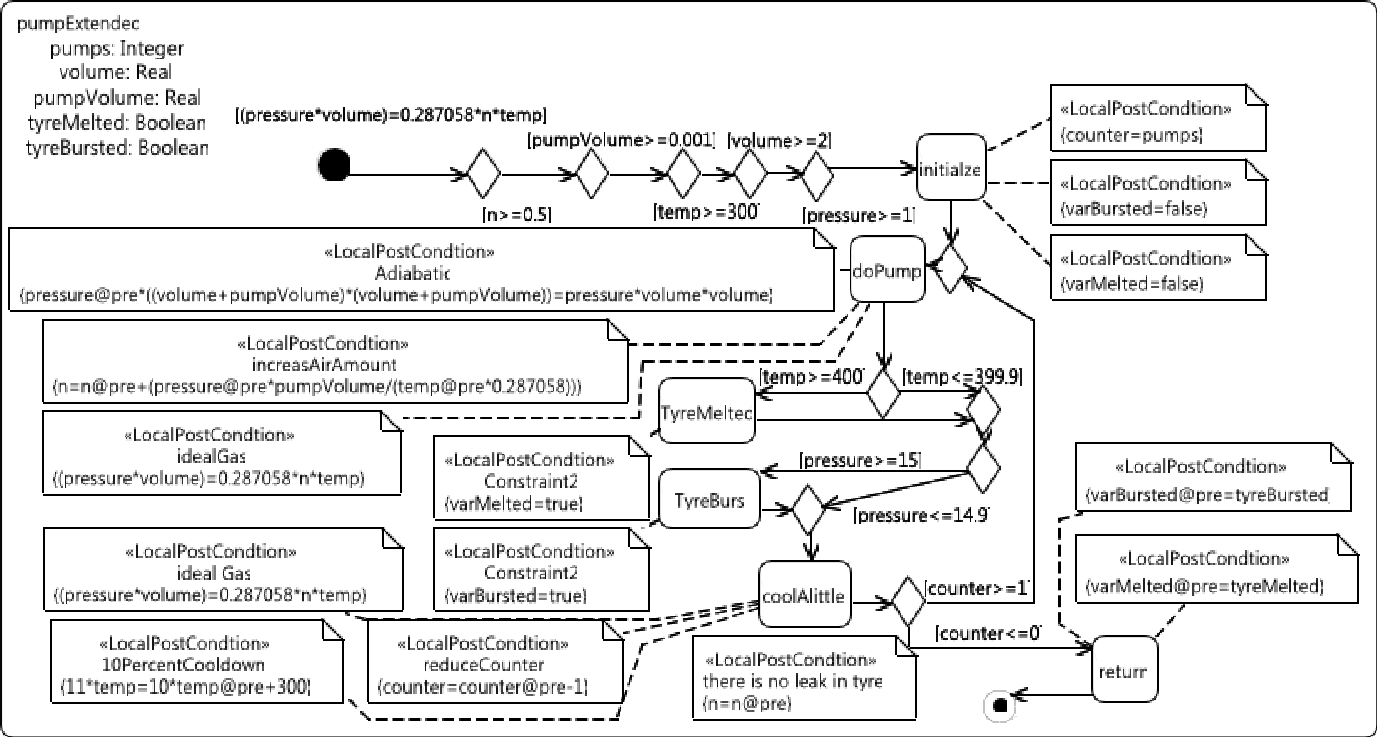
\includegraphics[width=\textwidth]{./pics/pumpTyre.pdf}
\caption{Activity Diagram with non convex mixed integer constraints}
\end{figure}
Figure \ref{fig:pumpTyre} shows an activity modelling the physical process of pumping air into a tyre. The realations between volume, amount of air ($n$), pessure, and temperature are described by the ideal gas equation. The equations for adiabatic compression of air during one pump strocke states a non-convex relation between these physical meassures. Aditionaly we introducesd the boolean Variables tyreExploded and tyreMelted, which will be set when the preassure or temperature inside the tyre rised above a certain threshold. Moreover we introduce an integer loop counter that determines how many pump strokes will be executed.\\
This model requires non-convex mixed integer problems to be solved in order to generate test data. The solver couenne from the coin-OR project is suitable for this task. We have implemented the modelled function in C and successfully ran the generated test cases against it. In Figure \ref{fig:ExplosionRuntime} we see the result of our experiment measuring the runtime of the testgeneration depending on the maximum length of control flow paths.\\
Non--convex mixed integer programs are in general undecidable consequently it may happen that a solver trying to solve an instance of an MIP runs infinitelly long. Couenne is the only solver we tested for non convex mixed integer constraint formulations. It ususally uses less than one minute to generate a feasible solution for one problem instance. But it also might run for a very long time or even infinitely long. Consequently we need to set a suitable time limit after which the solver shall terminate and we assume the currently examined control flow path as infeasible. When the timelimit is choosen verry small the test generation is faster but on the other hand we will also consider several paths as infeasible although there would be a solution for the corresponding problem instance. When setting a larger time limit to we will certainly find a solution more often and thus generate more Test cases but the overall runtime will grow. In Figure \ref{fig:ExplodingTyresRuntime} we decpict the overall runtime of the test generation for this model using couenne varying the the maximum path length and the time limit for one problem instance. On the right hand side of the Figure we depict the amount of test case found depending on the time limit and the maximum path length.

% \subsubsection{Constraint Programming}
% ILOGCP, Gecode or transformation possible
% \paragraph{Integer arithmetic only} Gecode
% \paragraph{linear mixed Integer arithmetic} IlogCP
% \begin{figure}
% \label{fig:classifyTriangle}
% 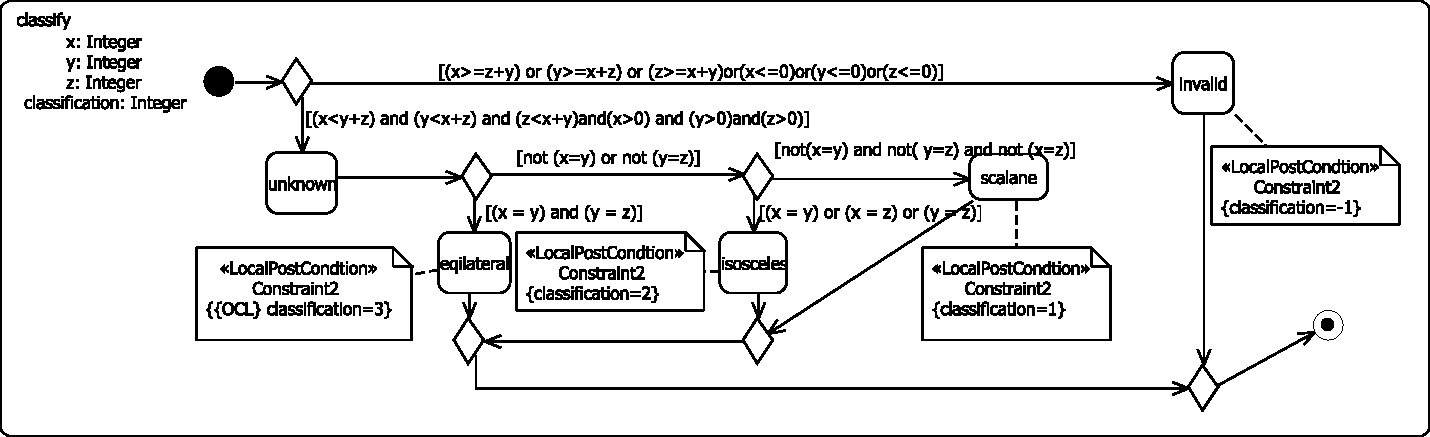
\includegraphics[width=\textwidth]{./pics/TriangleClassificator.pdf}
% \caption{Activity Diagram with non convex mixed integer constraints}
% \end{figure}
% \paragraph{nonlinear mixed Integer arithmetic}
% really really really problematic. Currently the only way is to transform the Activity Test Case Graph to remove the Logical Operations in favour of parallel or sequential Control Flows with guards. Use COUENNE.
\subsection{Case Study PAX Model}
\label{sec:evaluationCaseStudy}
We tested our implementation on a model modelling the PAX call system from Airbus. Out of the model of the complete product we selected an activity diagram modelling the interaction of the PAX call system with the \textbf{I}n \textbf{F}light \textbf{E}ntertainment (IFE) system. The selected \UMLType{Activity} contains 21 \UMLType{Actions}, 24 \UMLType{ControllNodes}, and two \UMLType{LoopNodes}. Furthermore there are eight \UMLType{DataStoreNodes} representing function local variables. The model was originally created with Artisan Studio, and used to generate a C-implementation from it with a proprietary code generator from Atego\textsuperscript{\textregistered}. The branching conditions and the code body of each \UMLType{Action} is given in C--syntax. All assignments and conditions consist of linear equations and inequalities only; thus the constraint satisfaction problem to be solved for test data generation is a linear program.\\
The described algorithm has several parameters, which mainly influence the \nameref{sec:pathsearch}. We use this case study to evaluate the influence of those parameters on the runtime of the Algorithm. The examined parameters are the maximum length of control flow paths to be tested, the maximum amount of test cases to be generated, and the frequency at which the early infeasible path check is performed during the path search.
\subsubsection{Manual Adaptation}
In order to generate C++ unit test code with our Eclipse plug-in from the described model several pre-processing steps need to be performed manually. Those manually to perform steps are the conversion of the Model from Atego\textsuperscript{\textregistered } Artisan Studio into Eclipse UML, adding all constraints in OCL syntax, the guards and the local post--conditions, flattening the \UMLType{LoopNodes}, and replacing the \UMLType{DataStoreNodes} by \UMLType{Properties}.\\
Atego\textsuperscript{\textregistered} does not store models natively in xmi format but has an option for exporting models in xmi format. The Eclipse Modelling Framework natively uses the xmi format to store models. Each modelling tool uses its own implementation of the UML meta model and there are slight differences in the implementations making the created models incompatible with each other. In order to import the model from Artisan in Eclipse we manually need to remove some objects not recognised by Eclipse and correct some typing errors in the xmi file. Then we can load the XMI and browse the model with the Eclipse Modelling Framework.\\
Every \UMLType{Action} is associated with a C-code snippet that is used for code generation. There are not yet \UMLType{Constraints} specifying the pre and post--conditions of each \UMLType{Action} in OCL. Also the \UMLReference{guards} do not contain OCL queries. We make an educated guess to add \UMLReference{guards} and \UMLReference{localPostconditions} reproducing the semantics of the C-code snippets contained in the original model. The original model used local C-struct variables modelled by the \UMLType{DataStoreNodes} contained by the \UMLType{Activity}. Our implementation can handle primitive data type variables modelled by \UMLType{Properties}, consequently we created one \UMLType{Property} per field of a struct variable. The original model also used arrays. We emulated the behaviour of an indexed collection by allowing all variables depending on an index to change to an arbitrary value whenever the index is changed. This may produce wrong behaviour but seemed fair enough to evaluate our algorithm. The \UMLType{DataStoreNodes} will be ignored by our algorithm.\\
The \UMLType{LoopNodes} contain further model elements in their \UMLReference{bodyPart} reference. Those elements from the \UMLReference{bodyPart} are directly included into the parent \UMLType{Activity} the \UMLType{InitialNode} and \UMLType{FinalNodes} of the loop body are replaced by decision nodes and directly connected to every element that was connected to the \UMLType{LoopNode}. In order to preserve the loop semantic a control flow from every final node of the body to the initial node of the body is added and decorated with a \UMLReference{guard}.\\
The function specifying which control flow to take after each \UMLType{Action} is \emph{well--defined} and \emph{defined} over the complete domain. Well--defined means there is no possible state in which more than one guard evaluates to true, and defined over the complete domain means that there is no value assignment for which all guards of the outgoing \UMLType{ControlFlows} evaluate to false.
\subsubsection{Runtime Experiments}
\begin{figure}
\begin{tikzpicture}
\begin{axis}[
width=0.49\textwidth,
legend style={at={(0.02,0.98)},anchor=north west},
ylabel={time},
xlabel={max path length},
ytick={10000000000,60000000000,600000000000,3600000000000},
yticklabels={10s,1m,10m,1h},
ymajorgrids=true,
yminorgrids=true,
xmajorgrids=true,
no markers,
ymode=log,
]
\addplot table[x=PATHSEARCH_MAX_PATHLENGTH,y=time(ns)]{Experiment-DATA/CaseStudyRuntimeCplex.csv};
\addlegendentry{Cplex};
\addplot table[x=PATHSEARCH_MAX_PATHLENGTH,y=time(ns)]{Experiment-DATA/CaseStudyRuntimeLPSolve.csv};
\addlegendentry{lpSolve};
\end{axis}
\end{tikzpicture}%
\begin{tikzpicture}
\begin{axis}[
width=0.49\textwidth,
xlabel={unchecked steps},
ylabel={time},
ytick={10000000000,60000000000,600000000000,3600000000000,864e11},
yticklabels={10s,1m,10m,1h,1d},
no markers,
legend style={legend columns=3,overlay,at={(0.5,1.02)},anchor=south},
ymajorgrids=true,
yminorgrids=true,
xmajorgrids=true,
xminorgrids=true,
no markers,
ymode=log,
] 
\addplot table[x=PATHSEARCH_UNCHECKED_STEPS,y=time(ns);]{Experiment-DATA/CaseStudyUncheckedSteps40.csv};
\addlegendentry{40};
\addplot table[x=PATHSEARCH_UNCHECKED_STEPS,y=time(ns);]{Experiment-DATA/CaseStudyUncheckedSteps50.csv};
\addlegendentry{50};
\addplot table[x=PATHSEARCH_UNCHECKED_STEPS,y=time(ns);]{Experiment-DATA/CaseStudyUncheckedSteps60.csv};
\addlegendentry{60};
\addplot table[x=PATHSEARCH_UNCHECKED_STEPS,y=time(ns);]{Experiment-DATA/CaseStudyUncheckedSteps70.csv};
\addlegendentry{70};
\addplot table[x=PATHSEARCH_UNCHECKED_STEPS,y=time(ns);]{Experiment-DATA/CaseStudyUncheckedSteps80.csv};
\addlegendentry{80};
\addplot table[x=PATHSEARCH_UNCHECKED_STEPS,y=time(ns)]{Experiment-DATA/CaseStudyUncheckedSteps90.csv};
\addlegendentry{90};
\end{axis}
\end{tikzpicture}%
%\end{center}
\caption{Runtime of Test Generation }
\label{fig:RuntimeExperiments}
\end{figure}
The implemented algorithm has several properties influencing the exact execution of the \nameref{sec:pathsearch}. In this section we will examine the influence of these parameters on the number of unit tests generated and the runtime of the algorithm. As already explained in Section \ref{sec:pathsearch} and Section \ref{sec:EarlyInfeasiblePathRecognition} there are two parameters that ensure the termination of the \nameref{sec:pathsearch}. Those are the maximal pathlength and the maximum amount of test cases generated. It is quite obvious that the number of test cases found may depend exponentially on the maximal control flow path length. We assume, that the path search algorithm described in Section \ref{sec:pathsearchDFS} will find abstract test cases at a constant rate. According to this assumption the runtime of the algorithm should linarly depend on the amount of test cases generated. Thus the maximal number of test cases to be found should be correlated linearly to the overall runtime of the algorithm, and we expect the maximum control flow path length to be exponentially correlated to the runtime of the test generation algorithm. \\
There is also one parameter steering the early infeasible path elimination. That is the amount of unchecked steps. Calling the solver is verry expensive in terms of runtime. To check wheather the current control flow path is infeasible we need to solve the corresponding constraint satisfaction problem. If we check everytime one control flow has been added to a control flow path we will eliminate infeasible paths as soon as possible, but will also call the solver unecessaryly often to find out that one constraint added did not make the path infeasible. If we perform a check for infeasible control flow paths after every tenth decision passed we will have to check at least $2^10$ control flow paths wheather they are feasible or not, where several of them could have been eliminated much earlier by computing much less constraint satisfaction problems. We pay special interrest to the influence of the number of unchecked decissions before control flow paths are checked for feasiblility. We assume, that there will be a minimum of runtime for some number of unchecked decissions.

%Complex data types we added one \UMLType{Property} per field in a variable.

%When the Model was correctly imported we need to add to each \UMLType{Action} those local post--conditions that describes the assignments done in the C-code associated with that \UMLType{Action}



I could do a case study with the Airbus PAX call model from Atego\textsuperscript{\textregistered }.
\section{Verification of the Implementation}
We claim that the Eclipse plug--in built aside this thesis implements the algorithm explained in \nameref{chap:testgeneration}. This claim is validated manually by checking each step separately. We use the Academic Example models presented in Section \ref{sec:evaluationAcademicModels} as test cases to verify each transformation described in \nameref{chap:testgeneration}. From each input model we created manually the intermediate artefacts that should have been created according to the specification and compared them to the intermediate artefacts produced by the plug-in.
\section{Limitations}
\label{sec:evaluationLimitations}
\subsection{Theoretical Limitations}
undecidability of nonlinear arithmetic over infite sets and Exponential runtime for Constraint solving algorithms for some formulations
\subsection{Limitations of the Implementation}
no structured activity nodes, no invariants, not completely implemented test goal management.
\subsection{Limitations of used Tools}
XMI interchange format does not work always LOTS OF BUGS!!!!
\subsubsection{AMPL}
\label{sec:LimitationsAMPL}
\section{further Ideas}
There is no good reason for using OCL as the specification language in order to ease the constraint solving prolog could directly be used as language to specify constraints in a UML Model.


